% !TEX root = main.tex

%------------------------------------------------
\chapter[Complex Numbers and Functions]{Preliminaries on Complex Numbers and Functions}


\subsection{Basic Definitions and Algebraic Operations}



Formally, a \emph{complex number} is an ordered pair $(x,y)$ of real numbers\marginpar{Of course, we want to say that a complex number $z$ is a number of the form $z=x+iy$ where $x,y \in \R$ and $i^2=-1$.  However, it is not so clear that the expression $x+iy$ makes sense yet.}.  We denote the set of all complex numbers by $\mathbb{C}$, and define addition and multiplication on $\C$ as follows:
\begin{enumerate}
\item[(i)] $(x_1,y_1)+(x_2,y_2) = (x_1+x_2,y_1+y_2)$,
\item[(ii)] $(x_1,y_1)(x_2,y_2) = (x_1x_2-y_1y_2,x_1y_2+x_2y_1)$.
\end{enumerate}
With this definition, $\C$ and $\R^2$ are equal \emph{as sets}, however, we have also defined an operation of multiplication on $\C$.


The subset of $\C$ given by 
\[
\set{(x,0): x \in \R } 
\]
is called the \emph{real axis}.  For complex numbers in this subset we have
\begin{align*}
(x_1,0)+(x_2,0) & = (x_1+x_2,0) \\
(x_1,0)(x_2,0) &= (x_1x_2,0), 
\end{align*}
so these complex numbers behave exactly like real numbers.  For this reason, we shall use $\R$ to refer to the real axis and denote the complex number $(x,0)$ by $x$.



Writing $i=(0,1)$, the definition of multiplication in $\C$ gives $i^2=-1$. With this notation, we get a more familiar `definition': a complex number $z=(x,y)$ can be written as
\begin{align*}
z = (x,y) &= (x,0)+(y,0)(0,1) \\
& = x + iy.
\end{align*}

The real numbers $x$ and $y$ are the \emph{real} and \emph{imaginary} parts of $z$ respectively, and we often write
\[
\Re (z) = x,\quad \Im (z)=y.\footnote{Note that the imaginary part of $z$ is \emph{real}}
\]

  The real and imaginary parts of $z$ are uniquely determined by $z$ in the following sense:
\[
\text{ for } w,z \in \mathbb{C}, w=z \text{ if and only if } \Re (z) = \Re (w) \text{ and } \Im (z) = \Im (w).
\]


With this more familiar notation, the algebraic operations of addition and multiplication on $\mathbb{C}$ can be expressed as follows: for $z_1=x_1+iy_1$ and $z_2=x_2+iy_2 \in \mathbb{C}$, we have
\begin{align*}
z_1 +z_2  &= (x_1+x_2) + i (y_1+y_2) \\
z_1z_2 & = (x_1+iy_1)(x_2+iy_2) \\
& = x_1x_2 + i (x_1y_2) + i (y_2x_2) + (i)^2(y_1y_2) \\
& = (x_1x_2-y_1y_2) + i (x_1y_2-x_2y_1).
\end{align*}








It is convenient to identify the complex number $z \in \C$ with the point (or sometimes, the vector) $(\Re (z), \Im (z) ) \in \R^2$.  Obviously the map $z \mapsto ( \Re (z), \Im (z))$ is a bijection $\C \to \R^2$, and thus geometrically, we view $\C$ as $\R^2$.




\begin{definition}[Complex Conjugate]
Given $ z \in \mathbb{C}$, the \emph{complex conjugate} $\overline{z}$ of $z$ is defined as
\[
\overline{z} := \Re (z) - i \Im (z). 
\]
\end{definition}

\begin{definition}[Modulus]
Given $z \in \mathbb{C}$, we define the modulus of $z$ to be
\[
| z | : = \sqrt{ \Re (z)^2 + \Im (z)^2 }.
\]
\end{definition}
\
In other words, for $z=x+iy$, $\conj{z}=x-iy$ and $\abs{z} = \sqrt{x^2+y^2}$.


Geometrically, the complex conjugate of $z$ describes the reflection of $z$ through the real axis, and the modulus of $z$ is the distance of $z$ from the origin.
Note that $| z | = \sqrt{\overline{z}z}$.




\begin{proposition}
Let $r \in \R, z, w \in \C$ be given.\marginpar{You really should be familiar with all of these properties.  I would suggest trying to prove at least some of them, or verifying them for some specific choices of $z$ and $w$. Most of the proofs are short.}
Then:
\begin{enumerate}
%\item $i^2 = -1$.
\item[(i)] $\conj{\conj{z}} = z$.
\item[(ii)] $\conj{z+w} = \conj{z} + \conj{w}$.
\item[(iii)] $\conj{zw} = \conj{z}\ \conj{w}$.
\item[(iv)] $\conj{r} = r$.
\item[(v)] $\Re (z) = \displaystyle\frac{z + \conj{z}}{2}$.
\item[(vi)] $\Im (z) = \displaystyle\frac{z - \conj{z}}{2i}$.
\item[(vii)] $\abs{z} = 0$ if and only if $z = 0$.
\item[(viii)] $\abs{z + w} \leq \abs{z} + \abs{w}$ \emph{(Triangle Inequality)}.
\item[(ix)] $\abs{zw} = \abs{z} \abs{w}$.
\end{enumerate}
\end{proposition}


\begin{definition}[Argument]
The \emph{argument} of a complex number $z \neq 0$ is the angle $\arg (z)$ from the positive real axis to the vector representing $z$.  
\end{definition}
Note that there are typically many ways in which we can represent $\arg (z)$, since we identify any two angles that differ by an integer multiple of $2\pi$ with one another.  For instance, for (the complex number) $z=1$ any of the angles
\[
\ldots,-4\pi, -2\pi, 0, 2 \pi , 4\pi,\ldots
\]
are valid choices for $\arg (z)$.   Similarly, if we look at $z=-1-i$:
\begin{center}
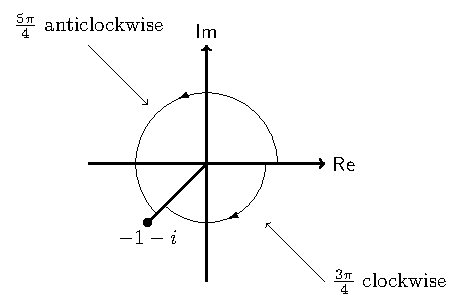
\includegraphics[scale=1]{arg}
\end{center}
We can write $\arg (z) = \frac{5\pi}{4}$ or $\arg (z)=- \frac{3\pi}{4}$ (or indeed an integer multiple of $2\pi$ added to either of these angles).




By convention we usually take $\arg (z) \in (-\pi , \pi]$.
\begin{definition}
For $z \in \C$, $z \neq 0$, we define the \emph{Principal argument of $z$} (or the \emph{Principal value of $\arg(z)$}) to be the value of $\arg (z)$ that lies in $(-\pi,\pi]$.{\marginpar{There was a typo here originally (missing minus sign in $(\pi,\pi]$)}}  We shall denote this value by $\Arg (z)$.
\end{definition}
So for $z=-1-i$ we have $\Arg (z) = - \frac{3 \pi}{4}$, while $\arg (z)$ can be taken to be any of the values
\[
\ldots, - \frac{11\pi}{4}, - \frac{3\pi}{4}, \frac{5\pi}{4}, \frac{13\pi}{4}, \ldots.
\]


\begin{definition}
The \emph{polar form} of a complex number $z$ is given by writing $z$ in the form
\[
z = r \left( \cos (\theta) + i \sin (\theta) \right),
\]
where $r , \theta \in \R$ and $r \geq 0$.
\end{definition}
The polar form of $z$ is found by setting $r = \abs{z}$ and $\theta = \arg (z)$ (any value of $\arg(z)$ will of course suffice). { Equivalently, we may write
\[
z = r e^{i \theta}
\]
(though we have yet to define the complex exponential function).}  For completeness, we should specify that the polar form of $0$ is simply $0$, since $\arg (0)$ is not defined.



\begin{definition}
Let $w=r \left( \cos( \theta) + i \sin ( \theta) \right)$ be (the polar form of) a complex number.  Then the $n^{th}$ \emph{complex roots} of $w$ are defined to be the $n$ solutions $\omega_0, \omega_1, \ldots , \omega_{n-1}$ of the equation $z^n = w$.  These roots are given by
\[
\omega_{k} = \sqrt[n]{r} \left( \cos \left( \frac{\theta+2k \pi}{n} \right) + i \sin \left( \frac{\theta + 2k\pi}{n} \right) \right),
\]
for $k=0,1,\ldots,n-1$, where $\sqrt[n]{r}$ is the (positive) $n^{th}$ real root of $r$.
\end{definition}


\begin{figure}[h]
\centering
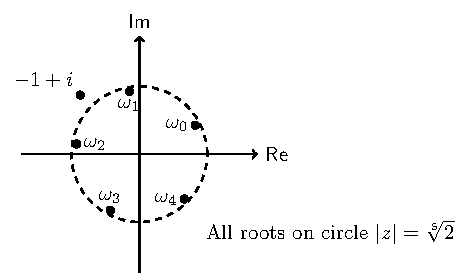
\includegraphics[scale=1]{sqrt1}
\caption{The 5\textsuperscript{th} roots of $z=-1+i$}.
\end{figure}




\begin{figure}[h]
\centering
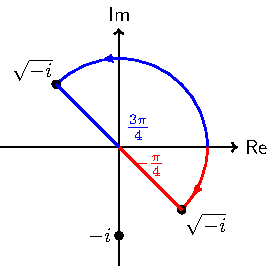
\includegraphics[scale=1]{sqrt}
\caption{The two square roots of $-i$}
\end{figure}

\begin{theorem}
Let $z_1$ and $z_2$ be nonzero complex numbers.  Then
\begin{enumerate}
\item[(i)] $\abs{z_1z_2}=\abs{z_1} \cdot \abs{z_2}$, and
\item[(i)] $\arg (z_1z_2)=\arg(z_1)+\arg(z_2)$.
\end{enumerate}
\end{theorem}
\begin{proof}
Exercise.
\end{proof}



\subsection{Complex Functions}

We now start our investigation of functions from the complex plane to itself.  First of all, note that a function $\mathbf{f}:\R^2 \to \R^2$ can be written in the form
\[
\mathbf{f}(x,y)=\left( u(x,y), v (x,y) \right)
\]
where $u,v:\R^2 \to \R$.  For example, if
\[
\mathbf{f}(x,y)=\left(x^2+y^2-2x,2y-6 \right),
\]
we have
\[
u(x,y)=x^2+y^2-2x \text{ and } v(x,y)= 2y-6.
\]





Since we have a formal definition of $\C$ as $\R^2$, we can express a function $f : \C \to \C$ as
\begin{equation*}
f(z) = f(x+iy) = u(x,y) +i v(x,y)
\end{equation*}
for all $z =x+iy \in \C$, where $u, v : \R^2 \to \R$. \ Equivalently, we could write
\[
f(z) = u(z) + i v(z),
\]
where $u,v: \C \to \R$.   In this way, we can extend our definition of real and imaginary parts from complex numbers to functions $f:\C \to \C$, writing $\Re (f) = u$ and $\Im (f) = v$.

{
\begin{itemize}
\item
Since we `define' $\C$ as $\R^2$, we can express a function $f : \C \to \C$ as
\begin{equation*}
f(z) = f(x+iy) = u(x,y) +i v(x,y)
\end{equation*}
for all $z =x+iy \in \C$, where $u, v : \R^2 \to \R$. 
\item Equivalently, we could write
\[
f(z) = u(z) + i v(z),
\]
where $u,v: \C \to \R$.  
\item Can extend our definition of real and imaginary parts from complex numbers to functions, writing $\Re (f) = u$ and $\Im (f) = v$.
\end{itemize}
}





Going in the other direction, given two functions $u:\R^2 \to \R$ and $v:\R^2 \to \R$, we can create a function $f : \C \to \C$ by \emph{defining} $f(x+iy) := u(x,y) +iv(x,y)$.
So,
\begin{center}
\emph{
 There is a correspondence between functions from the complex plane to itself, and pairs of functions from the real plane to the real line.}
 \end{center}




\begin{example}
The function \[ f: \C \to \C,\quad f(z) = \conj{z} \]
can be identified with 
\[ \mathbf{f}: \R^2 \to \R^2, \quad \mathbf{f}(x,y) = \left( u(x,y), v(x,y) \right)
\]
where
\begin{align*}
u(x,y) &= x \\
v(x,y) &= -y
\end{align*}
\end{example}
Since
\[
\conj{z} = \conj{x+iy} = x-iy = \underbrace{x}_{u(x,y)} + i \underbrace{(-y)}_{v(x,y)}.
\]


\begin{example}

Let us determine the functions $u:\R^2 \to \R$ and $v:\R^2 \to \R$ corresponding to
\begin{equation*}
h: \C \to \C, z \mapsto z^2.
\end{equation*}

{ We have
\[
(x+iy)^2 = x^2-y^2+i2xy
\]
Thus we identify $h:\C \to \C$ with $\mathbf{h}:\R^2 \to \R^2$, $\mathbf{h}(x,y) = (u(x,y), v(x,y))$  where
\begin{gather*}
u: \R^2 \to \R, (x,y) \mapsto x^2-y^2, \\
v: \R^2 \to \R, (x,y) \mapsto 2xy.
\end{gather*}
}
\end{example}


%\begin{master}
Substituting $x + iy$ for $z$ gives us
\begin{equation*}
z^2 = (x+i y)^2 = \underbrace{x^2-y^2}_{u(x,y)} +i\underbrace{ 2xy }_{v(x,y)}
\end{equation*}
%So the corresponding real function is
%\begin{equation*}
%h : \R^2 \to \R^2, (x,y) \mapsto (x^2-y^2, 2xy).
%\end{equation*}
Thus we identify $h:\C \to \C$ with $\mathbf{h}:\R^2 \to \R^2$, $\mathbf{h}(x,y) = (u(x,y), v(x,y))$  where
\begin{gather*}
u: \R^2 \to \R, (x,y) \mapsto x^2-y^2, \\
v: \R^2 \to \R, (x,y) \mapsto 2xy.
\end{gather*}
%\end{master}


\begin{example} Let us find the corresponding complex function, $f:{\mathbb C} \rightarrow {\mathbb C}$, for the function
\begin{equation*}
\mathbf{f} : \R^2 \to \R^2, (x,y) \mapsto (2y,-x)
\end{equation*}
and express it in terms of $z \in \C$.
\end{example}

%\begin{master}
\begin{solution}
The corresponding function $f:\C \to \C$ is given by
\begin{align*}
f(z)= f(x+iy)&=2y+i(-x) \\
& = 2 \Im (z) +i ( - \Re (z) ) \\
& = 2 \left( \frac{z-\overline{z}}{2i} \right)-i \left( \frac{z+\overline{z}}{2} \right) \\
&=\frac{-3i z}{2}+\frac{i\overline{z}}{2}.
\end{align*}

Thus the corresponding complex\marginpar{
Here we have used the identities $\Re (z) = \frac{1}{2} (z+\conj{z})$ and $\Im (z) = \frac{1}{2i}(z-\conj{z})$, together with the fact that $i^{-1}=-i$.
} function is
\begin{equation*}
f: \C \to \C, \ f(z)= \frac{-3i z}{2}+\frac{i\overline{z}}{2}.
\end{equation*}
\end{solution}
%\end{master}
%\vspace*{5cm}





\begin{example}
Let us do the same for the functions $\mathbf{f}:\R^2 \to \R^2$ defined by
\begin{enumerate}
\item[(i)] $\mathbf{f} (x,y) = (-2y+3,2x),$ and
\item[(ii)] $\mathbf{f}(x,y) = (x^2+y^2-2x,2y-6)$.
\end{enumerate}

\end{example}

\begin{solution}
We could follow the strategy of the previous example and use the fact that if $z=x+iy$ then
\begin{align*}
x & = \Re(z) = \frac{1}{2} \left( z+ \conj{z} \right) \\
y & = \Im (z) = \frac{1}{2i} \left( z- \conj{z} \right).
\end{align*}
Substituting these expressions for $x$ and $y$, we could then simplify and find $f(z)$. However, this is time consuming, and it is sometimes easier to look for familiar expressions in the definition of $f$.

In part (i), $\mathbf{f}$ corresponds to $f: \C \to \C$ defined by
\begin{align*}
f(z) = f(x+iy) &= -2y+3+i(2x) \\
& = 2(ix-y) + 3 \\
& = 2(ix+i^2y)+3 \\
& = 2i(x+iy)+3 \\
& = 2iz+3.
\end{align*}

In part (ii), $\mathbf{f}$ corresponds to $f:\C \to \C$ where
\[
f(x+iy) = x^2+y^2-2x+i2y-6i.
\]
With $z=x+iy$, notice that
\[
x^2+y^2=\abs{z}^2 = z \conj{z},
\]
and that
\[
-2x+i2y = -2 (x-iy) = -2 \conj{z},
\]
hence
\[
x^2+y^2-2x+i2y-6i = z \conj{z} - 2 \conj{z} -6i.
\]
Hence $f(z) = z \conj{z}-2\conj{z}-6i$ is the corresponding complex function.



\end{solution}

\begin{example}
Find the real and imaginary parts of the function $f:\C \to \C$, 
\[
f(z) = z^2-3z+4-7i.
\]
\end{example}

%\vspace*{10cm}
\begin{solution}
We are looking for $u,v:\R^2 \to \R$ so that $f(x+iy)=u(x,y)+iv(x,y)$.  To find them, we write
\[
z^2-3z+4-7i=(x+iy)^2-3(x+iy)+4-7i.
\]
After some simplification, separating into real and imaginary parts gives
\[
f(x+iy) = \underbrace{x^2-y^2-3x+4}_{u(x,y) \text{ or } \Re (f)}+i (\underbrace{2xy-3y-7}_{v(x,y) \text{ or } \Im (f)})
\]
\end{solution}


It is worth recalling that some familiar functions defined on $\R$ extend to $\C$.

\begin{definition}
\label{d:exp}
The \emph{exponential function} is the function $\exp : \C \to \C$ defined by
\[
\exp (x+iy) = \exp(x) \left( \cos (y) + i \sin (y) \right)
\]
for all complex numbers $x+iy \in \C$, where $\exp (x) (=e^x)$ is the usual (real) exponential of $x$.
\end{definition}
We shall often write $e^z$ in place of $\exp (z)$.   The trigonometric functions also extend to $\C$ via
\begin{align}
\cos (z) &= \frac{1}{2} \left( \exp (iz) + \exp (-iz) \right) \\
\sin (z) & = \frac{1}{2i} \left( \exp(iz)- \exp (-iz) \right).
\end{align}



Note that Definition~\ref{d:exp} justifies our alternative expression for the polar form of $z$.  Indeed, for any $\theta \in \R$ we have
\begin{align*}
\exp( i \theta ) =  \exp( 0+i \theta ) &= \exp (0) \left( \cos ( \theta) + i \sin (\theta) \right) \\
& = \left( \cos ( \theta) + i \sin (\theta) \right).
\end{align*}
Hence writing $z=r \left( \cos(\theta) + i \sin ( \theta ) \right)$ ( $r,\theta \in \R$ and $r>0$) is equivalent to writing\marginpar{\textbf{Note:} Since we do not yet know how to raise a (real) number to a complex power, it is not yet clear that $\exp(w+z)=\exp(w)\exp(z)$ and so on.  However, for the purposes of this module, you may assume that this identity is true (it is easily verified from the definition).}
\[
z = r \exp (i \theta).
\]



We conclude this section with some remarks about how you might go about `visualising' a complex function.  For functions $f:\R \to \R$, we usually do so by drawing the graph of $f$, that is, the subset $\set{(x,f(x)): x \in \R}$ of $\R^2$.

We cannot draw the `graph' of a function $f:\C \to \C$, as to do so would require four coordinates
\[
\set{ \Re (z), \Im (z) , \Re \left( f(z) \right), \Im \left( f(z) \right) }
\]
and thus four dimensions.  We can however view $f$ as a `transformation' of the complex plane, and examine the effect of applying $f$ to
\begin{itemize}
\item Regions (subsets) of $\C$
\item Curves in $\C$ (lines, circles etc)
\item A combination of the two.
\end{itemize}


\begin{figure}[h]
\centering
{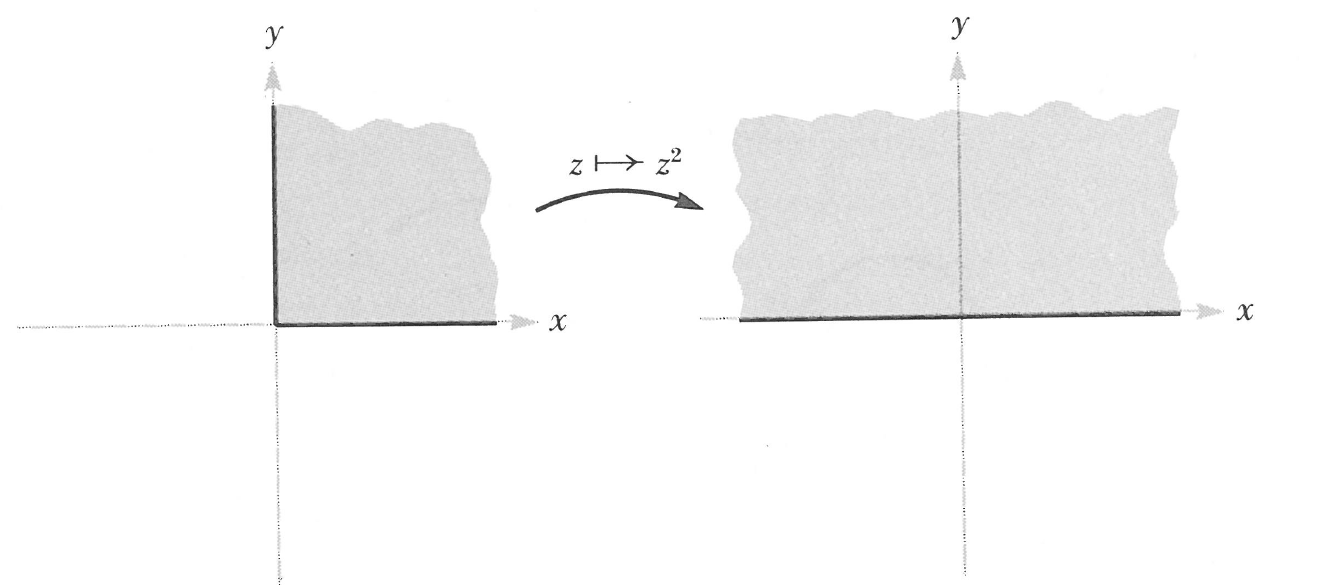
\includegraphics[scale=0.4]{z2quad}}
{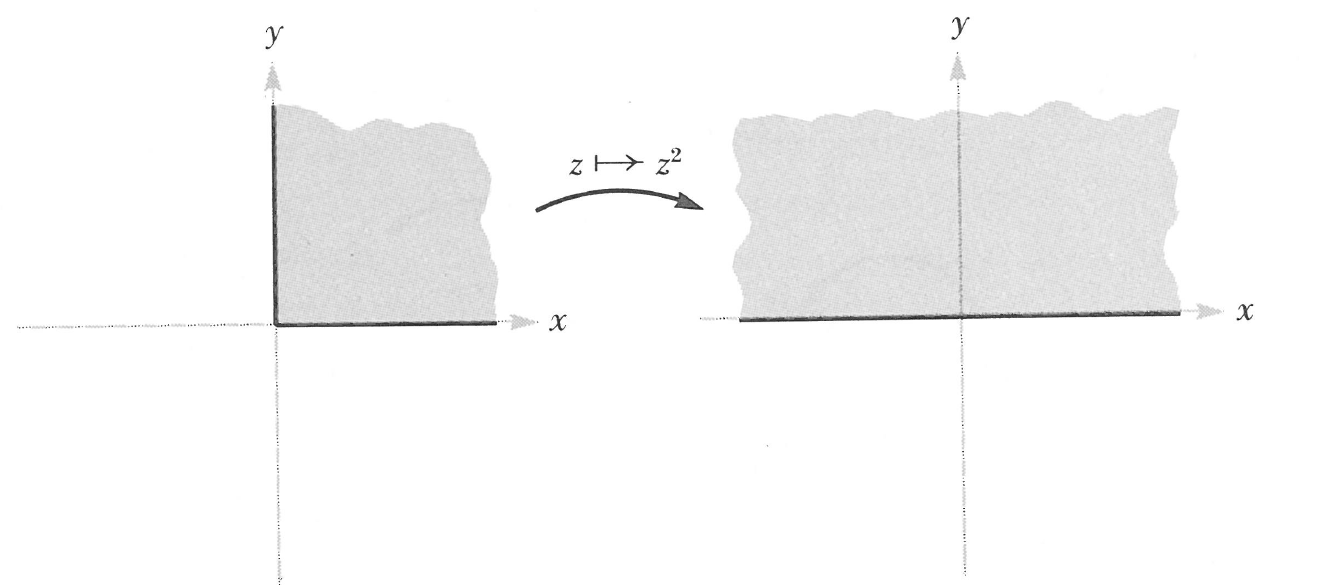
\includegraphics[scale=0.25]{z2quad}}
\caption{The image of the first quadrant under $z \mapsto z^2$.}
\label{f:z2}
\end{figure}
Figure~\ref{f:z2} indicates that the image of the first quadrant under the map $z \mapsto z^2$ is the region consisting of the first and second quadrants.  This follows from the fact that for any $z_1,z_2 \in \C$, 
\[
\arg (z_1z_2)=\arg(z_1)+\arg(z_2).
\]
Hence $\arg(z^2)=2\arg(z)$, and so if $0 \leq \arg (z) \leq \pi/2$ (i.e. $z$ is in the first quadrant), we have $0 \leq \arg (z^2) \leq \pi$ ($z^2$ lies in either the first or second quadrant).  Of course, Figure~\ref{f:z2} does not tell us anything about the modulus of $z^2$.


Figure~\ref{f:z2c} illustrates how $z \mapsto z^2$ also squares the modulus; the circle of radius $r>0$ and centre $0$ is sent to the circle of radius $r^2$ and centre $0$.  Moreover, the anticlockwise arrows on the circles indicate that if $z_2$ lies (a small distance) anticlockwise of $z_1$, then $z_2^2$ lies anticlockwise of $z_1^2$.




%\vspace*{2cm}

\begin{figure}[h]
\centering
{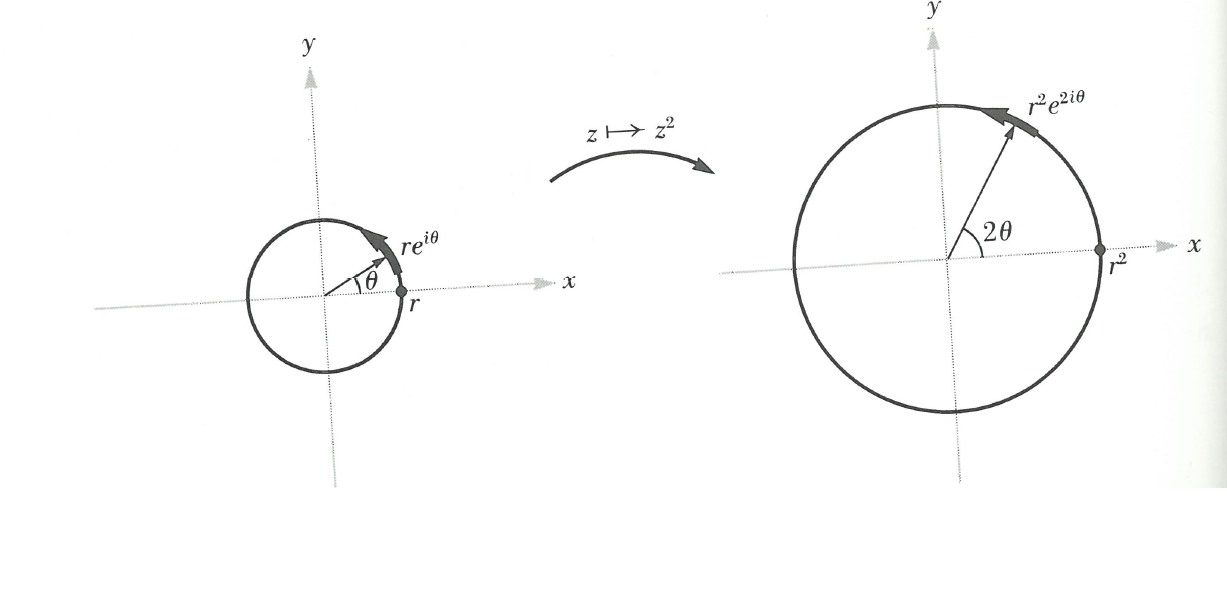
\includegraphics[scale=0.5]{z2circle}}
{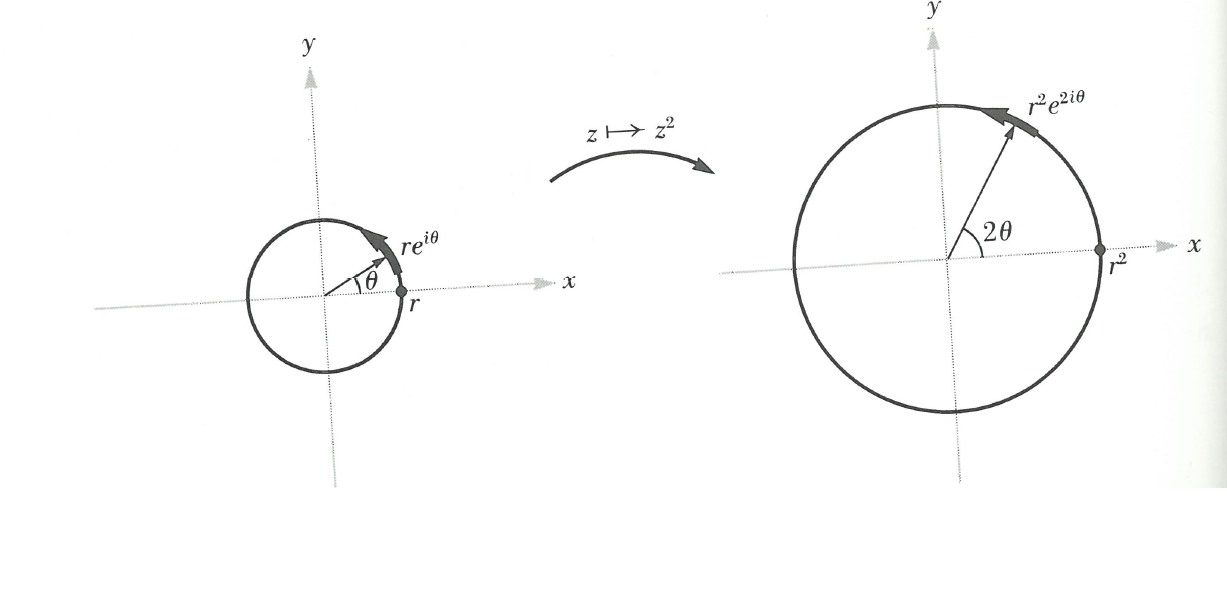
\includegraphics[scale=0.25]{z2circle}}
\caption{The effect of the map $z \mapsto z^2$ on a circle of radius $r$ centred at the origin.}
\label{f:z2c}
\end{figure}

%\vspace{2cm}

\begin{figure}[h]
\centering
{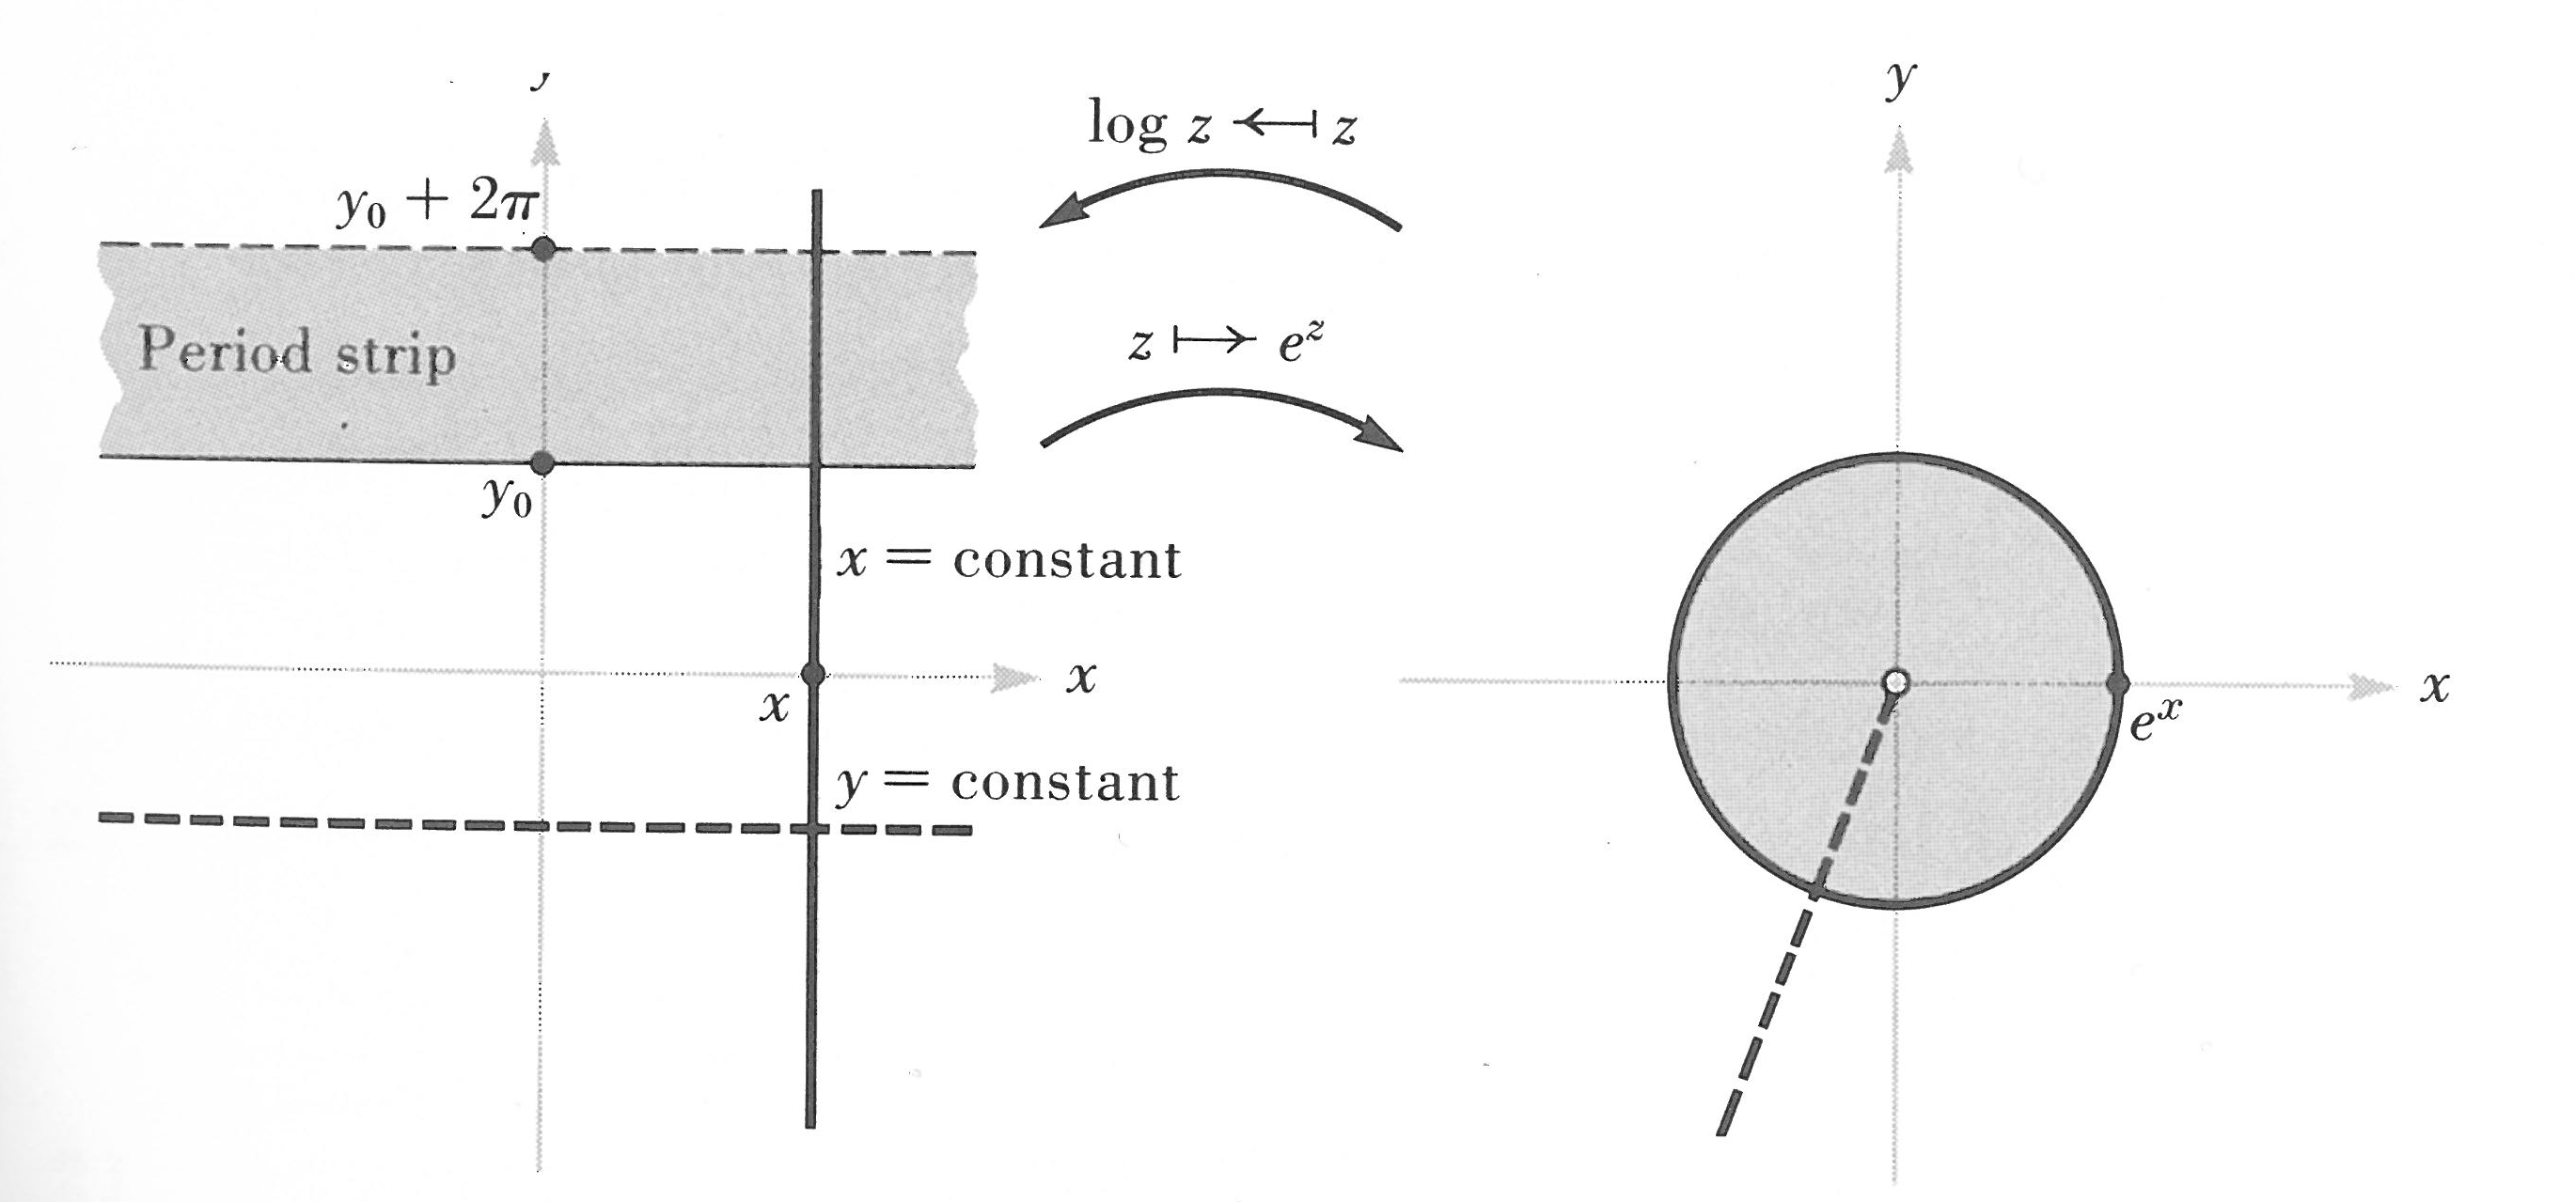
\includegraphics[scale=0.25]{expimage}}
{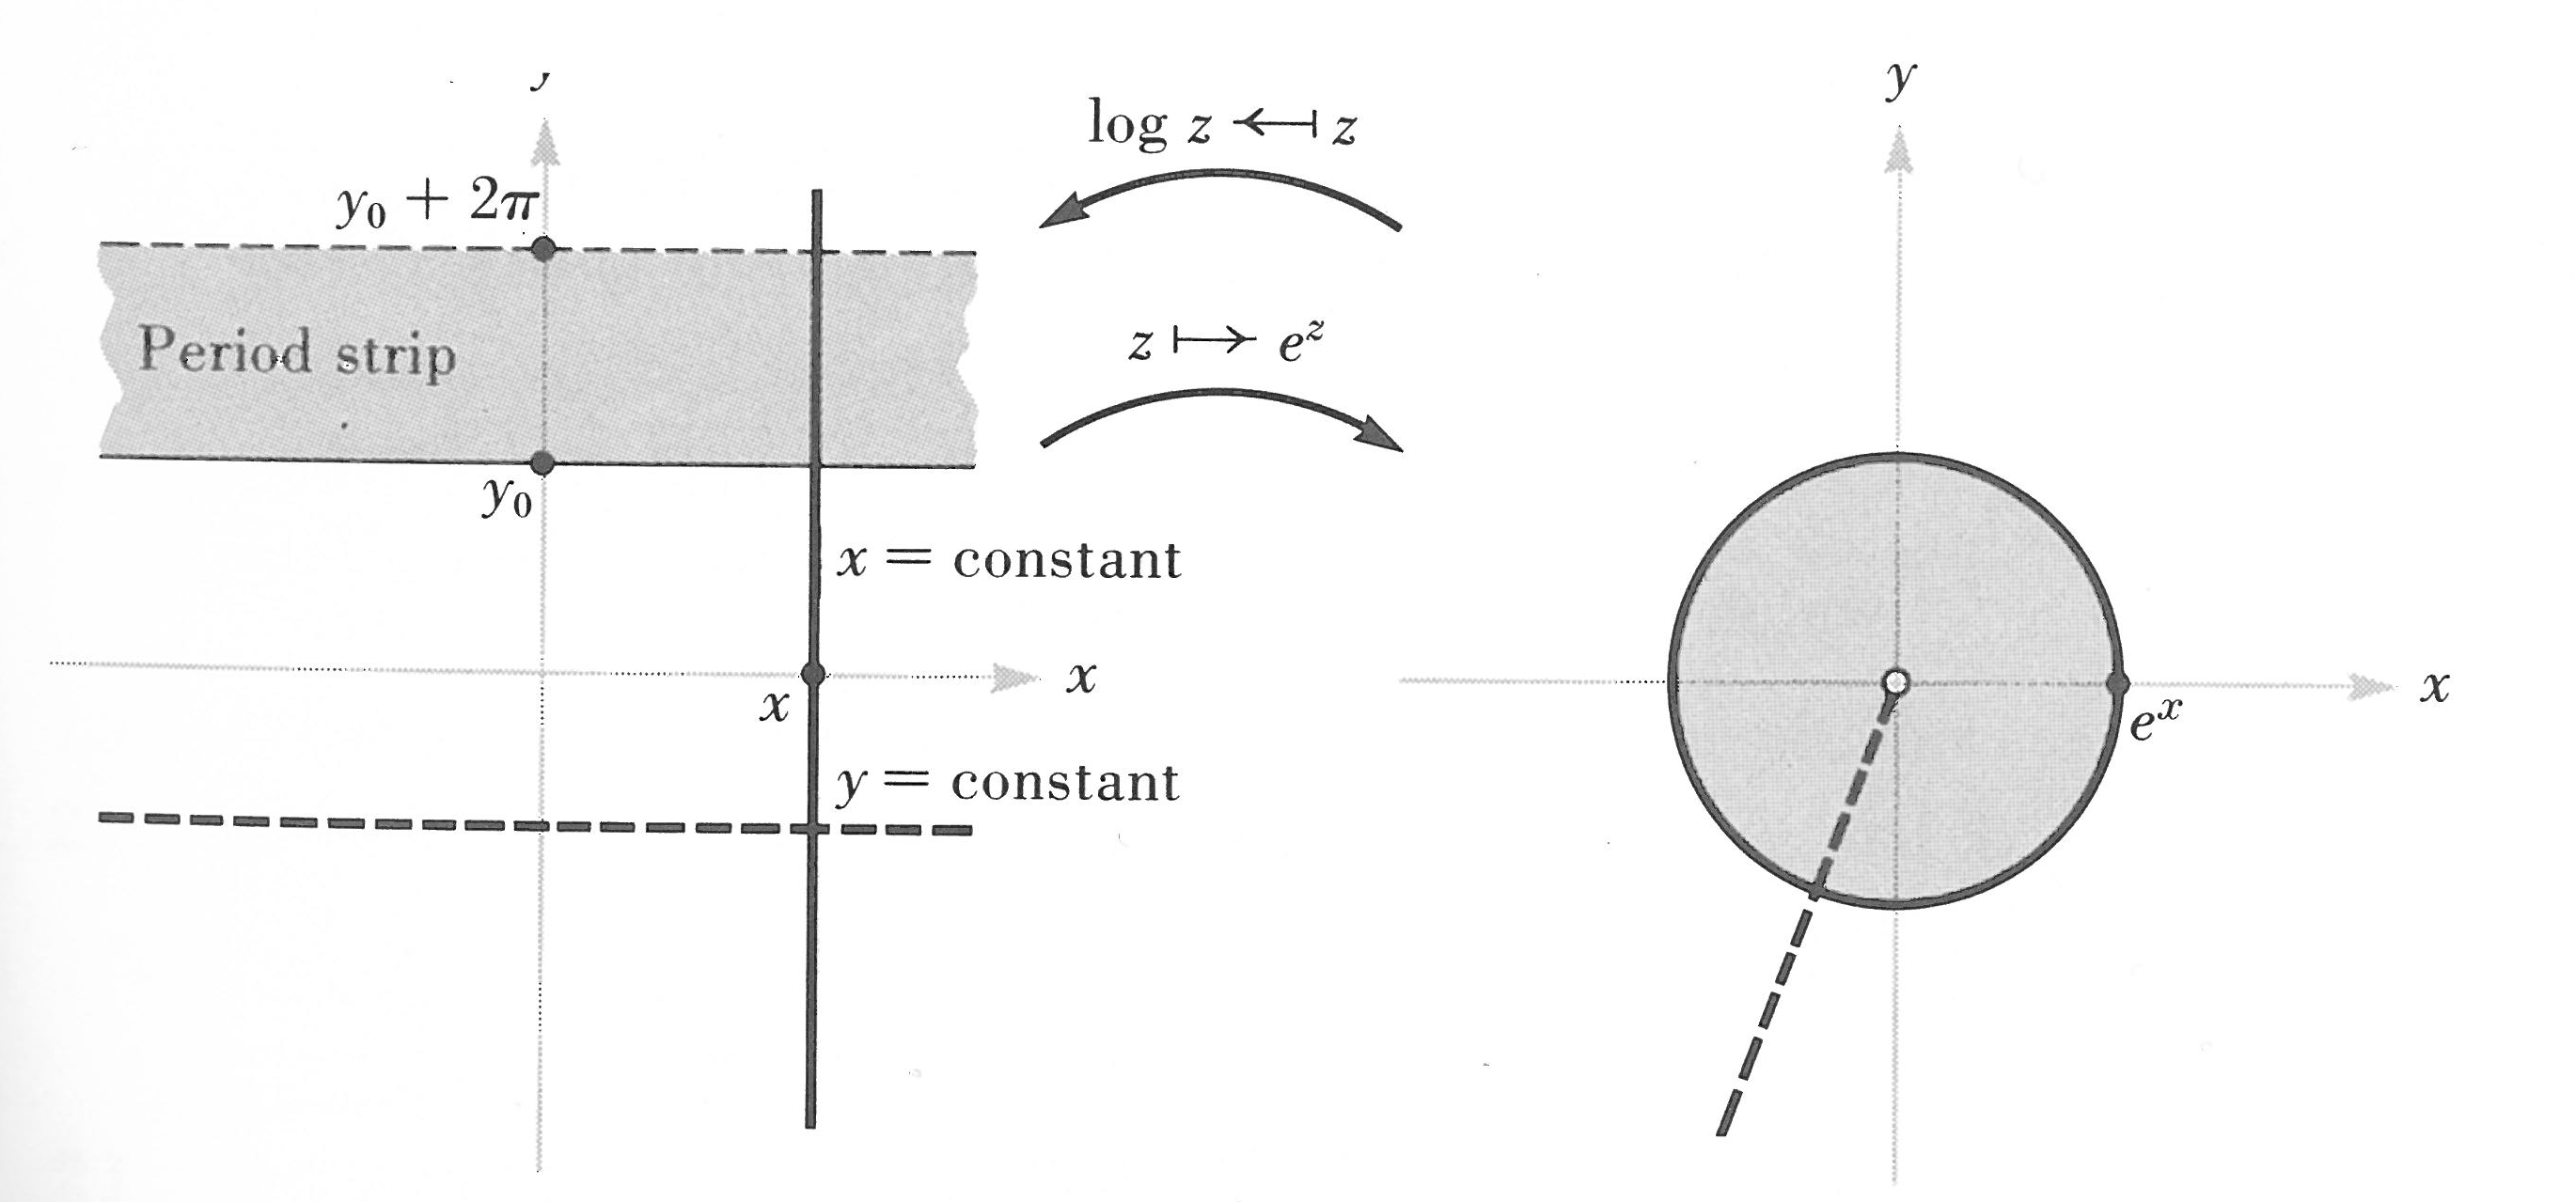
\includegraphics[scale=0.125]{expimage}}
\caption{The geometric effect of the exponential map.}
\label{f:exp}
\end{figure}

Figure~\ref{f:exp} combines the approaches of the previous examples.\marginpar{Strictly speaking this diagram is inaccurate, as some of the region to the right of the line $\Re(z)=x$ is also shaded}  Here we see that the shaded region,
\[
\set{z \in \C: \Re (z) \leq x \text{ and } y_0 \leq \Im (z) < y_0+2\pi}
\]
is sent to the shaded disc of radius $e^x$ and centre $0$.  The vertical line $\Re(z)=x$ is sent to the circle of radius $e^x$ and centre $0$, while the dashed horizontal line is sent to the `infinite ray' from $0$ indicated with another dashed line.
%\vspace{2cm}

\begin{figure}[h]
\centering
{
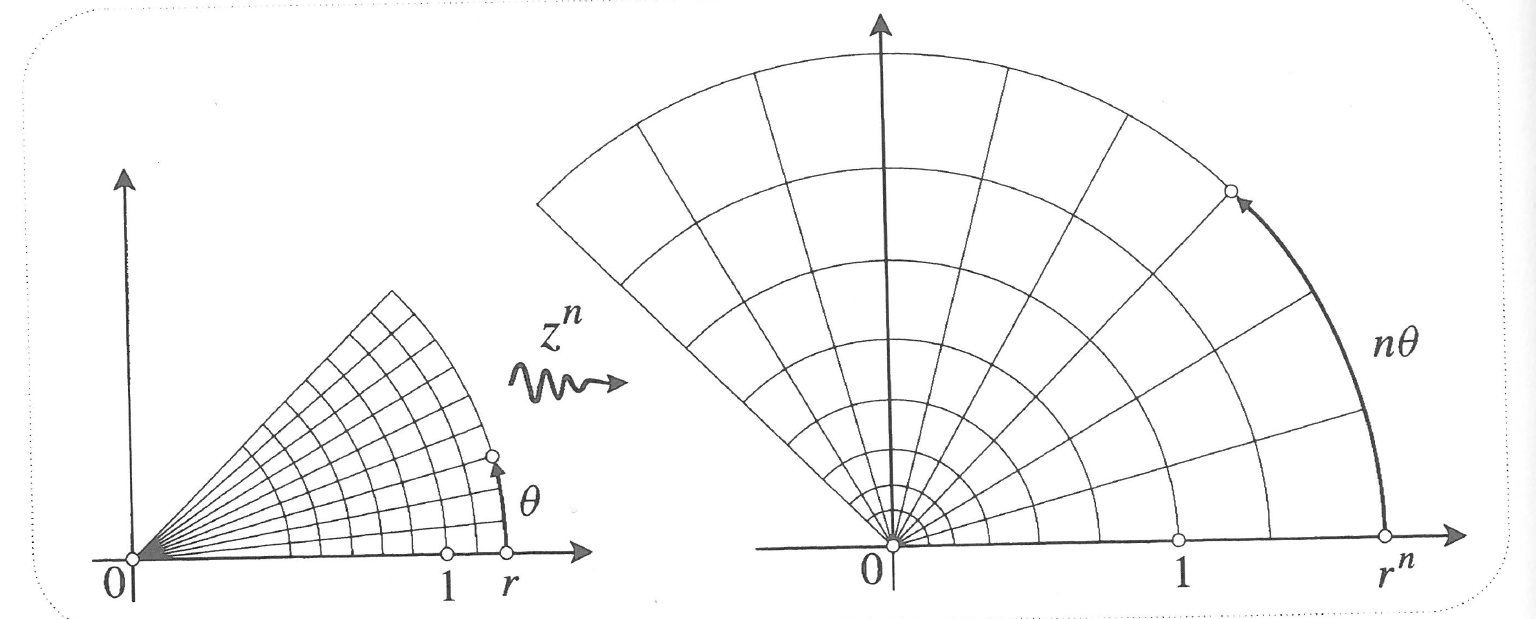
\includegraphics[scale=0.35]{znmap}
}
{
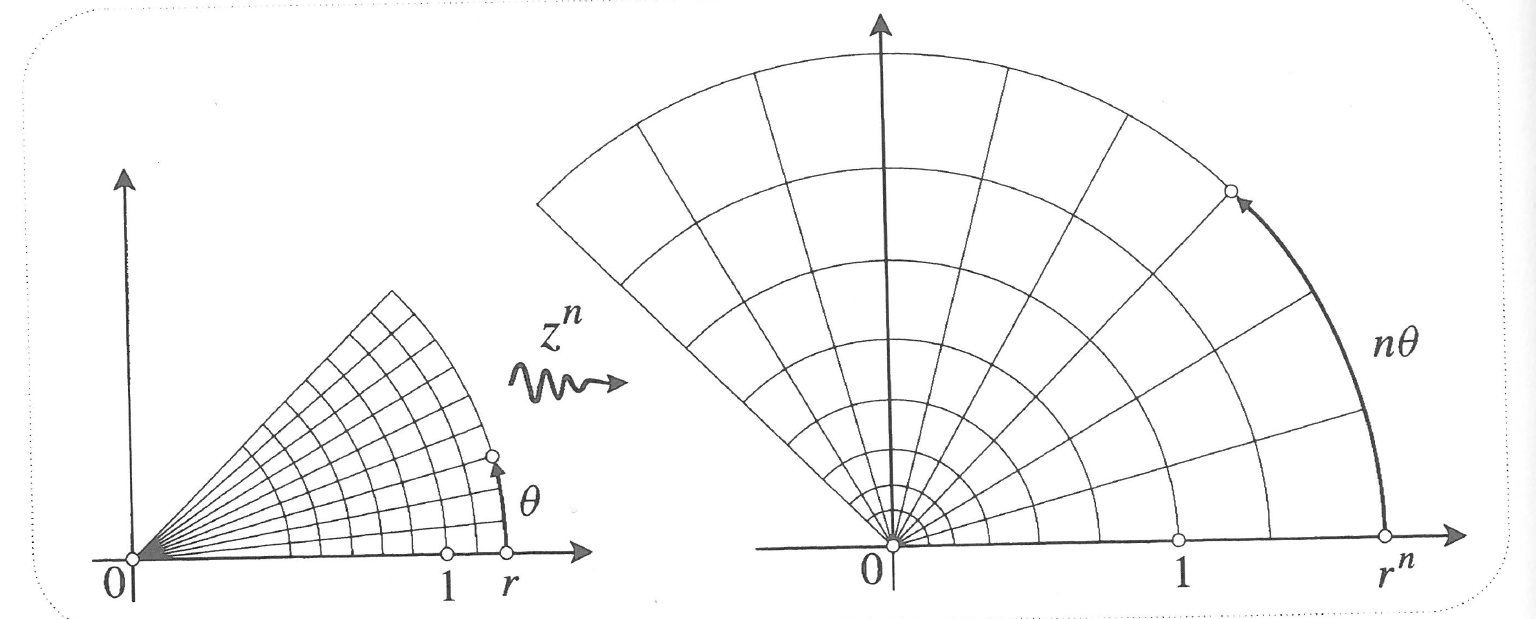
\includegraphics[scale=0.25]{znmap}
}
\caption{Another representation of $z \mapsto z^n$.  Note how this diagram indicates that the map $z \mapsto z^n$ shrinks the region $\abs{z}<1$ and enlarges the region $\abs{z}>1$.}
\label{f:zn}
\end{figure}

%\vspace*{2cm}
%Figures~\ref{f:z2},~\ref{f:z2c} and~\ref{f:exp} are from \emph{Basic Complex Analysis}, (Jerrold. E. Marsden, published by W.H. Freeman and Company, 1973).  Figure~\ref{f:zn} is from \emph{Visual Complex Analysis}, (Tristan Needham, published by Oxford University Press, 1997).

% !TEX root = main.tex

%------------------------------------------------
\section{Open Sets in $\C$}




\begin{definition}[Open Disc]
Let $w \in \C$ and let $r>0$ be some real number.  The open disc of radius $r$ centred at $w$ is defined to be the set 
\[
D(w,r):= \set{ z \in \C: \abs{z-w} <r}.
\]
\end{definition}
In other words, $D(w,r)$ is the set of all points that lie (strictly) inside the circle or radius $r$ with centre $w$.
\begin{definition}
The set of points
\[
D'(w,r) = \set{ z \in \C: 0 < \abs{z-w} < r},
\]
where $r>0$ and $w \in \C$, is called the \emph{punctured open disc} of radius $r$, centre $w$.\marginpar{This is a good place to introduce some conventions for sketching sets.  The broken circle in Figure~\ref{f:discs} around the disc indicates that the boundary is not included in this set.  The filled point $\bullet$ beside $w$ indicates that the point $w$ is included in $D(w,r)$, while the `hollow' point $\circ$ beside $w$ indicates that $w$ is not included in the punctured disc $D'(w,r)$.}
\end{definition}


Note that $D'(w,r)$ is the set obtained by removing the centre $w$ from the open disc $D(w,r)$.
\begin{figure}[h]
\centering
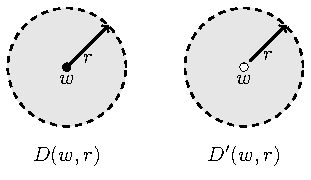
\includegraphics[scale=1]{discs}
\caption{The open disc $D(w,r)$ and punctured open disc $D'(w,r)$.}
\label{f:discs}
\end{figure}



\begin{definition}
Let $U \subseteq \C$, then we say that $U$ is an \emph{open set} if given any $w \in U$ there is some $r_w>0$ with $D(w,r_{w}) \subseteq U$.
\end{definition}
\begin{figure}[h]
\centering
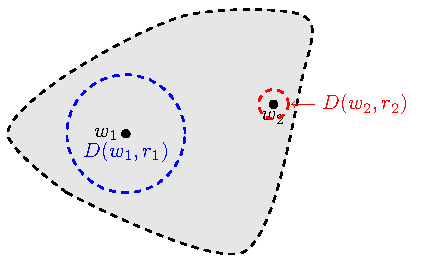
\includegraphics[scale=1]{openset}
\caption{An open set $U$ with two examples of open discs around points of $U$.  Note that the radius typically depends on the point $w$; points nearer the `edge' of $U$ will need smaller discs.}
\end{figure}



\begin{figure}[h]
\centering
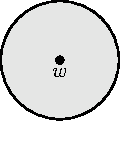
\includegraphics[scale=1]{cldisc}
\caption{An example of a set that is not open.  If we take any point $z$ on the boundary and any $r>0$, the open disc $D(z,r)$ contains points outside of the set.}
\label{f:discs2}
\end{figure}
\marginpar{The solid circle in Figure~\ref{f:discs2} indicates that the boundary is included}


\begin{example}
 The open disc $D(0,1)$ is an open set.

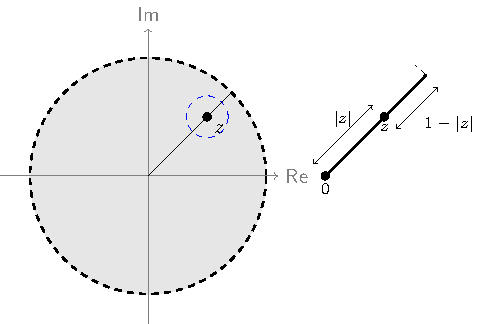
\includegraphics[scale=1]{unit_disc_full}


Let $z \in D(0,1)$.  Our goal is to find some $r>0$ so that $D(z,r) \subseteq D(0,1)$. and set $r= (1-\abs{z})/2$. Then if $w \in D(z,r)$,
\begin{align*}
\abs{w-0} & \leq \abs{w-z} + \abs{z} \\
& < \frac{1-\abs{z}}{2} +\abs{z} \\
&= \frac{1+\abs{z}}{2} < \frac{1+1}{2} = 1,
\end{align*}
which shows that $w \in D(0,1)$.

%\vspace*{2cm}


Hence $D(z,r) \subseteq D(0,1)$ and so $D(0,1)$ is open.

\end{example}



\begin{example}
 The upper-half plane $H_+$, where
\[
H_+ := \set{ z \in \C: \Im (z) > 0 }
\]
is an open set.
\begin{center}
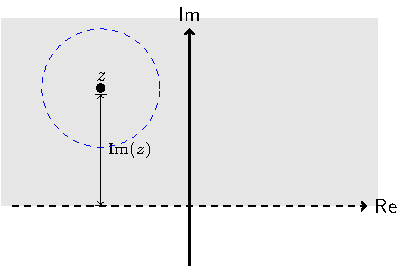
\includegraphics[scale=1]{upperhalf_full}
\end{center}
If $z \in H_+$ then $\Im (z)>0$, so we set $r = \frac{1}{2} \Im (z)$.  We want to show that $D(z,r)\subseteq H_+$, or in other words, given any $w \in D(z,r)$, we must have $\Im(w)>0$.

Let $w \in D(z,r)$, then
\[
\abs{\Im(z)-\Im(w)} \leq \abs{z-w} < r= \frac{\Im (z)}{2}.
\]
If $\Im(w)\leq 0$ then since $\Im(z)>0$ we would have
\[
\abs{\Im(z)-\Im(w)} = \Im(z) + \abs{\Im (w) } \geq \Im (z) > \frac{1}{2} \Im (z),
\]
which is a contradiction.  Hence $D(z,r) \subseteq H_+$ as required.

\end{example}



\begin{example} 
The lattice
\[
\mathbb{Z} + i\mathbb{Z} : = \set{ n + im: n,m \in \mathbb{Z} }
\]
is not open.
\begin{center}
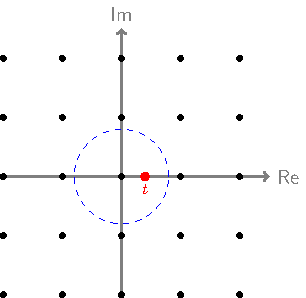
\includegraphics[scale=1]{lattice_full}
\end{center}

%\vspace*{12cm}
We shall show that the point $0 \in \mathbb{Z}+i \mathbb{Z}$ has the property that for any $r>0$, the disc $D(0,r)$ contains points in the complement of $\mathbb{Z}+i \mathbb{Z}$.\marginpar{To show that a set $S \subseteq \C$ is \emph{not} open, it is enough to find a single point $w \in S$ with the property that for any $r>0$, $D(w,r) \cap \left( \C \backslash S \right) \neq \emptyset.$}

Indeed, for any $r>0$ the point $t+0i$ where $t=\min ( \frac{1}{2} , \frac{r}{2} )$ belongs to $D(0,r)$ but not to $\mathbb{Z}+i\mathbb{Z}$.

\end{example}


\begin{note}
Some more examples of open sets include $\C \backslash \set{0}$, or indeed $\C \backslash F$ where $F$ is any finite set.  Many regions determined by \emph{strict} inequalities of real numbers are also open, for example, sets of the form
$
\set{ z \in \C: c_1<\abs{z}<c_2 }$, $\set{ z \in \C: 0 < \Arg (z) < \pi/4 }$ or $\set{z \in \C: c_1<\Re(z) < c_2 },$
where $c_1<c_2 $ are real numbers.

More examples of sets that are not open include circles, lines, curves, single points or finite sets.\marginpar{Do not use \emph{closed} to mean \emph{not open}.  In the context of analysis, closed has a different meaning.}
\end{note}
Throughout this module, we shall be mostly concerned with functions $f:U \to \C$, where $U$ is an open subset of $\C$.  

 
\subsection{Limits}
Limits in $\C$ are defined in an analogous way to those in $\R$ (and almost identically to those in $\R^2$). 

First, fix some complex number $w \in \C$.  For any $z \in \C$, the modulus $\abs{z-w}$ measures the distance between $z$ and $w$.  Note that if we write $z=x+iy$ and $w=u+iv$, then $\abs{z-w}$ is exactly the same as the Euclidean distance between $(x,y)$ and $(u,v)$ in $\R^2$.




 For a complex function $f$, what does it mean to say that $f$ approaches $L \in \C$ as $z$ approaches $w$?  \ Intuitively, we want
 \begin{center}
 $\abs{f(z)-L}$ is small whenever  $\abs{z-w}$ is small.
 \end{center}
  More formally, this can be written as
 \begin{center}
 Given any $\epsilon>0$ there is a $\delta>0$ such that
 \[
 \abs{f(z)-L} < \epsilon\text{ whenever } \abs{z-w}<\delta.
 \]
 \end{center}
 
 This definition works whenever $f$ is defined on all of $\C$, but it is not so clear how it should work when $f(z)$ is not defined near $w$. \marginpar{In other words, we want to be able to exclude points $w$ where $\abs{z-w}$ small implies $f(z)$ does not exist.} 
 
 
 \begin{definition}
 A point $w$ is a \emph{limit point} of of a set $S \subseteq \C$  if for any $\delta>0$, we have
 \[
 D'(w,\delta) \cap S \neq \emptyset.
 \]
 In other words, any punctured disc centred at $w$, no matter how small, contains at least one point of $S$.
 \end{definition}

A limit point of a set $S$ may or may not belong to $S$.  Moreover, a point $w \in S$ may or may not be a limit point of $S$.  \marginpar{If $S$ is an open set however, then any $w \in S$ is necessarily a limit point of $S$.}



\begin{example}
\begin{enumerate}
\item[(i)]  If $S=D'(w,r)$ is the punctured disc of radius $r>0$ centred at $w$, then $w$ is a limit point of $S$ that is not in $S$.
But if $R=D(w,r)$ is the complete disc, $w$ is a limit point of $R$ and $w \in R$.
\begin{center}
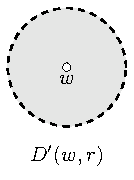
\includegraphics[scale=1]{pdisc}
\end{center}
In both cases, it is enough to note that for any $\delta>0$, the punctured disc $D'(w,\delta)$ either contains $D'(w,r)$, or else is contained in $D'(w,r)$.  In either case, the point $z:=w+s$, where $s=\min ( \frac{r}{2},\frac{\delta}{2})$ is contained in $D'(w,r) \cap D'(w, \delta)$.

\item[(ii)] If $S= \set{w}$ is a one-point set, then there are no limit points of $S$.  Indeed, for any $\delta>0$, $D'(w,\delta)$ does not contain any points of $S$ by definition.  Moreover, given any other point $z\in \C$ with $z \neq w$, the punctured disc $D'(z,\delta)$, with $\delta = \frac{1}{2} \abs{z-w}$, does not contain $w$.

\item[(iii)] The set of limit points of the open disc $S=D(w,r)$ is precisely the closed disc
\[
\set{z \in w: \abs{z-w} \leq r }.
\]
\begin{center}
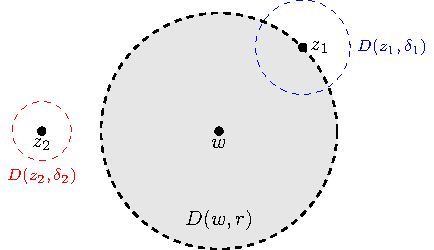
\includegraphics[scale=1]{opendisc_limitpoints} \qquad
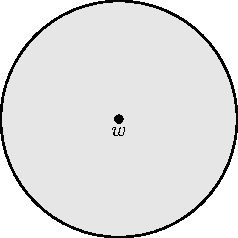
\includegraphics[scale=1]{cldisc_big}
\end{center}

If $z_1$ is a point on the boundary of $D(w,r)$, then for any $\delta>0$, $D'(z_1,\delta)$ contains points of $D(w,r)$.  If $z_2$ lies outside the boundary of $D(w,r)$, the the disc $D(z_2,\delta_2)$, where $\delta_2 = \frac{1}{2} ( \abs{w-z_2} -r)$, does not contain any points of $D(w,r)$.

\end{enumerate}
\end{example}


\begin{note}
To confuse things further, some authors require only allow points $w \in \C \backslash S$ to be limit points of $S$.  When reading textbooks or lecture notes, take care as to which definition is being used.
\end{note}


\begin{definition}
\label{d:limit}
Let $f$ be a complex function, $S \subseteq \C$ the domain of $f$,  and let $w \in \C$ be a limit point of $S$. Then we say that \[ \lim_{\substack{z \to w \\ z \in S}} f(z) = \alpha \in \C\] if given any $\epsilon >0$ there is some $\delta >0$ such that
\[ \text{ if $z \in S$ and } 0<\abs{z-w} < \delta \text{ then }\abs{f(z)-\alpha}< \epsilon.\]
\end{definition}
 
 

\begin{note}

\begin{enumerate}
\item[(i)]  Definition~\ref{d:limit} may equivalently be written in the language of open discs: 
\[
\lim_{\substack{z \to w \\ z \in S}} f(z) = \alpha
\]
if given any $\epsilon >0$ there is a $\delta >0 $ such that
\[
z \in D' (w, \delta ) \cap S \text{ implies } f(z) \in D( \alpha, \epsilon).
\]
\item[(ii)] When
\[ \lim_{\substack{z \to w \\ z \in S}} f(z) = \alpha \]
we sometimes write
\[
f(z) \to \alpha \text{ as } z \to w.
\]
\end{enumerate}

\end{note} 


\begin{example}
Is it possible to find a function $f$ for which $f(z) \to \alpha_1$ and $f(z) \to \alpha_2$ as $z \to w$, where $\alpha_1\neq\alpha_2$?
\begin{solution}
The answer, unsurprisingly, is no.  Indeed, set $\epsilon = \frac{1}{3} \abs{\alpha_1-\alpha_2}>0$.  If $f(z) \to \alpha_1$ and $f(z) \to \alpha_2$ as $z \to w$, then there would be some $\delta >0$ such that
\[
z \in D'(w,\delta) \Longrightarrow f(z) \in D'(\alpha_1 , \epsilon ) \cap D'(\alpha_2 , \epsilon).
\]
But this is impossible since clearly $D'(\alpha_1,\epsilon) \cap D'(\alpha_2 , \epsilon) = \emptyset$.
\end{solution} 
\end{example}
  
 
 
 
 \begin{comment}
This motivates our precise definition of a limit



\begin{example}
\begin{itemize}
Let $f(z)=z^3$ and $w=1+i$.
 
\end{itemize}
\end{example}

Note: it is not so clear how to adapt the definition of a limit to the case where the domain of $f$ is a proper subset of $\C$.  In order to do this, we will need to restrict our attention to a particular type of subset of $\C$ called an open set.

\begin{definition}[Limit of a function at a point of its domain]
Let $U \subseteq \C$ be an open set and $f: U \to \C$ a function defined on $U$.  For a point $w \in U$ we say that $\lim_{z \to w} f(z) = L$ if given any $\epsilon >0$ there is some $\delta >0$ such that for all $z \in U$ satisfying $\abs{z-w} < \delta$ we have $\abs{f(z)-L}< \epsilon$.
\end{definition}
We will need to generalise this definition slightly later on to allow for the case of $\lim_{z \to w} f(z)$ at a point $w \not\in \mathrm{dom} (f)$.  For example, we do not yet know how to calculate something like
\[
\lim_{z \to 0} \frac{\sin (z)}{z}
\]
(if it exists).
\end{comment}


\begin{proposition}[Algebra of limits] 
\label{p:alglimits}
Let $S\subseteq \C$ and consider functions $f,g:S \to \C.$  Suppose that $w$ is a limit point of $S$, and that $\displaystyle \lim_{\substack{z \to w \\ z \in S}} f(z) = \alpha$ and $\displaystyle \lim_{\substack{z \to w \\ z \in S}} g(z)= \beta$.  Then
\begin{enumerate}
\item[(i)] $\displaystyle \lim_{\substack{z \to w \\ z \in S}} \left( f(z) + g(z) \right) = \alpha + \beta$,
\item[(ii)] $\displaystyle \lim_{\substack{z \to w \\ z \in S}} \left( f(z)g(z) \right) = \alpha  \beta$,
\item[(iii)] If in addition $\beta \neq 0$, and $w$ is a limit point of the set $T=\set{ z \in S: g(z) \neq 0 }$, then
\[
\lim_{ \substack{z \to w \\ z \in T}} \frac{f(z)}{g(z)} = \frac{\alpha}{\beta}
\]
\end{enumerate}
\end{proposition}

\begin{proof}
The proof of this proposition is almost identical to the corresponding proof for real functions (except that $\abs{\cdot}$ refers to the modulus and not the absolute value), and is thus omitted.
\end{proof}
%\vspace*{3cm}


\subsection{Restricted Limits}

Suppose that $T$ is a subset of $S$ and $w$ is a limit point of both $T$ and $S$.  Then 
\[
 z \in D'(w, \delta) \cap T \text{ implies } z \in D' (w,\delta) \cap S.
\]
\begin{figure}[h]
\centering
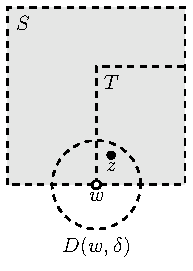
\includegraphics[scale=1]{subset1}
\caption{A subset $T$ of $S$ and a point $w$ that is a limit point of both $T$ and $S$.}
\end{figure}


It follows that
\[
 \lim_{\substack{z \to w \\ z \in S}} f(z) = \alpha \text{ implies }  \lim_{\substack{z \to w \\ z \in T}} f(z) = \alpha
\]

The second limit, where $f$ is restricted to the subset $T$ of $S$, is called a \emph{restricted limit}.   If a function has a limit at a point $w$ then all restricted limits of that function at $w$ must be the same.   In particular, 

\emph{If we have two subsets $T_1,T_2 \subseteq S$ such that 
\[
 \lim_{\substack{z \to w \\ z \in T_1}} f(z) = \alpha_1 \text{ and } \lim_{\substack{z \to w \\ z \in T_2}} f(z) = \alpha_2,
\]
with $\alpha_1 \neq \alpha_2$, then
\[
\lim_{\substack{z \to w \\ z \in S}} f(z)
\]
does not exist.
}



\begin{figure}[h]
\centering
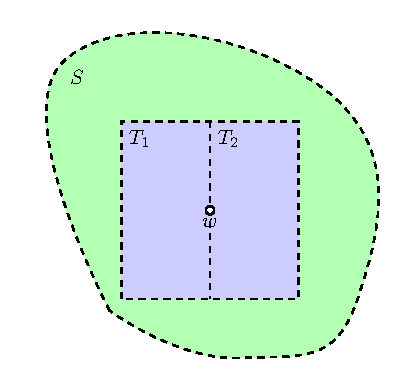
\includegraphics[scale=0.75]{subset2}\quad
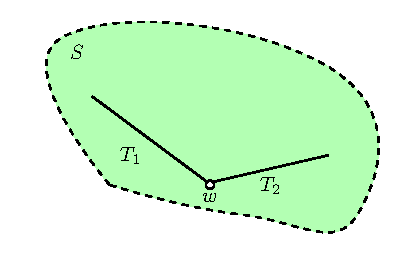
\includegraphics[scale=0.75]{subset3}
\caption{Examples of subsets $T_1$ and $T_2$ of $S$, and a common limit point $w$ of $T_1$ and $T_2$.  We shall often consider subsets of the type shown in the image on the right, where $T_1$ and $T_2$ are lines.}
\end{figure}



Let $f$ be a complex function with domain $S$ and let $w$ be a limit point of $S$.  In what follows, we shall simply write $\displaystyle \lim_{z \to w} f(z)$ in place of \[
\lim_{\substack{z \to w \\ z \in S}} f(z),
\]
and we shall reserve the second subscript for restricted limits.



\begin{example}
\label{e:rlim}
Consider the function 
\[
f: \C \backslash \set{0} \to \C, \quad f(z) = \frac{\conj{z}}{z}.
\]
Does 
$
\displaystyle \lim_{z \to 0} f(z)
$
exist?
\end{example}
\begin{note}
In future, we may simply write things like ``Let $f(z) = \dfrac{\conj{z}}{z}$'' without specifying the domain, since it is clear that this function $f$ is defined on $\C \backslash \set{0}$.
\end{note}

We shall look at two restricted limits of $f(z)$ as $z$ approaches $0$, namely the limits when $z$ is restricted to the subsets
\begin{itemize}
\item $\R \backslash \set{0}$, and
\item $i \R \backslash \set{0}$ \marginpar{Since every point on the imaginary axis is of the form $iy$ for some $y \in \R$, it makes sense to use the notation $i \R$ for this set.}
\end{itemize}
of the domain $\C \backslash \set{0}$.  Note that $0$ is a limit point of both $\R \backslash \set{0}$ and $i\R \backslash \set{0}$.
\begin{center}
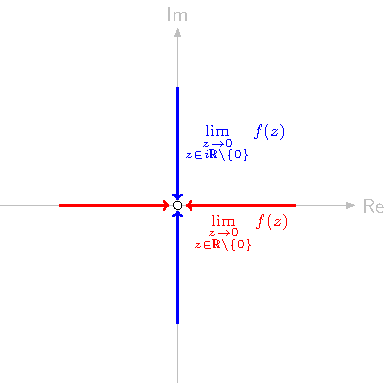
\includegraphics[scale=1]{origin_full}
\end{center}
If $z \in \R \backslash \set{0}$, then $\conj{z} = z$ and so $f(z) = \frac{\conj{z}}{z} = \frac{z}{z} =1$ on $\R \backslash \set{0}$.  Hence
\[
\rlim{z \to 0}{z \in \R \backslash \set{0} } f(z)=1.
\]
For $z \in i \R \backslash \set{0}$, we have $\conj{z}=-z$, so that $f(z)=-1$ for all such $z$, giving
\[
\rlim{z \to 0}{z \in i\R \backslash \set{0} }=-1.
\]
Since  these limits are not equal, it follows that the (unrestricted) limit $\lim_{z \to 0} f(z)$ does not exist.
%\vspace*{12cm}
\section{Continuity}

\begin{definition}
Let $S \subseteq \C$ and let $f:S \to \C$ be given.  For a point $w \in S$\marginpar{Note that the definition of continuity at $w$ only makes sense when $w$ belongs to the domain of $f$}, we say that $f$ is \emph{continuous at $w$} if $\lim_{z \to w } f(z)=f(w)$. If $f$ is continuous at all points $w \in S$ then we say that $f$ is \emph{continuous on $S$}.
\end{definition}



\begin{example}
\label{e:cts}

The functions
\begin{enumerate}
\item[(i)] $f(z) = \Re (z)$,
\item[(ii)] $f(z) = \Im (z)$, and
\item[(iii)] $f(z) = \conj{z}$
\end{enumerate}
are all continuous on $\C$.
\end{example}

\begin{solution}
Fix $w=x_0+iy_0 \in \C$ and let $\epsilon>0$ be given.  Note that for any $z=x+iy \in \C$ we have the following inequalities:
\begin{align*}
\abs{ \Re (z) - \Re (w)} = \abs{\Re (z-w)} & = \sqrt{(x-x_0)^2} \\
&\leq \sqrt{(x-x_0)^2+(y-y_0)^2} = \abs{z-w} \\
\abs{ \Im (z) - \Im (w)} = \abs{\Im (z-w)} & = \sqrt{(y-y_0)^2} \\
&\leq \sqrt{(x-x_0)^2+(y-y_0)^2} = \abs{z-w} \\
\abs{\conj{z}-\conj{w}} = \abs{\conj{z-w}} & = \abs{z-w}.
\end{align*}
Thus in all three cases, setting $\delta=\epsilon$, we get
\[
0< \abs{z-w} < \delta \Longrightarrow \abs{f(z)-f(w)} < \epsilon.
\]
\end{solution}



\begin{proposition}
\label{t:continuity}
Let $S \subseteq \C$ and let $f,g:S \to \C$ be functions that are continuous on $S$.  Then
\begin{enumerate}
\item[(i)] The function $f+g,$ where $(f+g)(z)=f(z)+g(z)$, is continuous on $S$,
\item[(ii)] The function $fg$, where $(fg)(z):=f(z)g(z)$, is continuous on $S$,
\item[(iii)] For any $\alpha \in \C$, the function $\alpha f$, where $(\alpha f)(z)=\alpha \left( f(z) \right),$ is continuous on $S$,
\item[(iv)] If $T=\set{z \in S: g(z) \neq 0 }$ then the function $ f/g$, where $ \left( \dfrac{f}{g} \right) (z)= \dfrac{f(z)}{g(z)},$ is continuous on $T$.
\end{enumerate}
\end{proposition}
\begin{proof}
Immediate from Proposition~\ref{p:alglimits}.
\end{proof}

\begin{note}
If we have
\[
f(x+iy) = u(x,y) + i v(x,y),
\]
and $w = x_0 + i y_0$ is a point in the domain of $f$, then
\[
\lim_{z \to w} f(z) = \lim_{(x,y) \to (x_0,y_0)} u(x,y)+ i \lim_{(x,y) \to (x_0,y_0)} v(x,y),
\]
provided these limits exist.  Hence
\[
f \text{ continuous at }w \Leftrightarrow u \text{ and } v \text{ continuous at } (x_0,y_0).
\]
This is useful when the real and imaginary parts of $f$ are familiar functions that we know to be continuous.
\end{note}



%------------------------------------------------
\endinput


